\documentclass{article}

\usepackage{tikz,pgfplots}
\usepackage[utf8]{inputenc}
\usetikzlibrary{positioning}

\title{Tikz}
\author{Aditya Yadav}

\begin{document}

\maketitle
\section{Drawing graphics}
\subsection{Drawing Lines}
\tikz \draw (0,0)--(2,1)--(3,2);
\tikz \draw (2,7)--(2,4)--(1,5);

\subsection{Drawing Circles}

\begin{itemize}
\item Circle with center at 0,0 and radius 1 cm\\
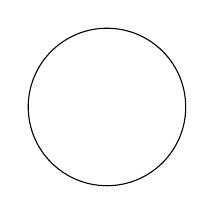
\begin{tikzpicture}
    \draw (0,0) circle (1);
\end{tikzpicture}
    
\item Another circle with center at 2,0 and radius 1 inches\\
\begin{tikzpicture}
    \draw (2,0) circle (1in);
\end{tikzpicture}
\end{itemize}

\subsection{Drawing Ellipse}
Ellipse with center at (3,0) and radiis are 10pt and 20pt\\
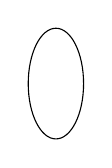
\begin{tikzpicture}
    \draw (3,0) ellipse (10pt and 20pt);
\end{tikzpicture}

\subsection{Drawing Rectangles}
Rectangle with left corner at 0,0 and bottom right corner at 5,4\\
\begin{tikzpicture}
	\draw (0,0) rectangle (5,4);
\end{tikzpicture}

\subsection{Drawing a grid}
Grid with left corner at 0,0 and bottom right corner at 5,4\\
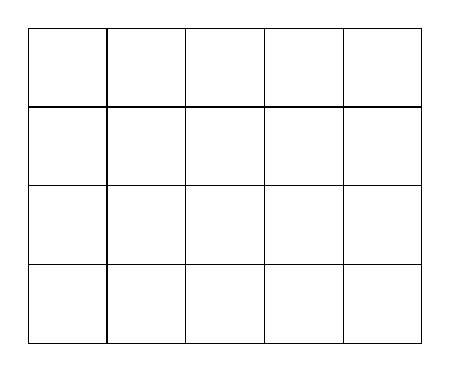
\begin{tikzpicture}
	\draw (0,0) grid (5,4);
\end{tikzpicture}

\subsection{Drawing arcs}
arcs have a syntax of start\_angle : stop\_angle : radius\\
\begin{tikzpicture}
	\draw (0,0) arc (30:60:3);
	\draw[dashed] (0,0)--++(30+180:3) -- +(60:3);
\end{tikzpicture}
\begin{tikzpicture}
	\draw (0,0) arc (60:180:6);
	\draw[dashed] (0,0)--++(60+180:6) -- +(180:6);
\end{tikzpicture}

\subsection{Drawing an arrow}
\begin{tikzpicture}
	\draw[->] (0,0)--(3,3);
\end{tikzpicture}

\subsection{Drawing text at a position}
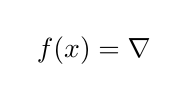
\begin{tikzpicture}
	\draw node at (0,0) {$f(x)=\nabla$};
\end{tikzpicture}

\subsection{Labeling a figure}
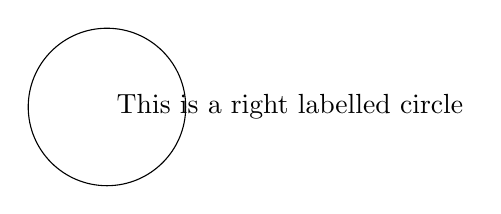
\begin{tikzpicture}
	\draw (0,0) circle (1) node[anchor=west]{This is a right labelled circle};
\end{tikzpicture}
\end{document}